\documentclass[11pt,letterpaper]{article}
\usepackage[margin=1in]{geometry}
\usepackage{graphicx}
\usepackage{hyperref}
\usepackage{listings}
\pagestyle{headings}
\usepackage{epstopdf}

\begin{document}

\title{PHY 410 \\ Homework Assignment 3}
\author{Han Wen \\ \tiny Person No. 50096432}
\date{\today}

\maketitle

\begin{abstract}
The goal of this assignment was to develop a thorough understanding of Fourier Transform and FFT.
\end{abstract}

\tableofcontents

\newpage
\section{Problem 1}

\subsection{Description}
Run the Lecture 6 fft test code and interpret the power spectrum. What is the period of the oscillations? What N does this correspond to? How do you convert? 




\subsection{Solution}
Here is the result plotting ~\ref{figure1} . We can see from the original code or from the power we can see the frequency is 10. And the function of the plot is 
$y=sin(-\frac{2\pi fx}{N})$.

Therefore period $T=\frac{N}{f}=102.4$

 
\begin{figure}
\begin{center}
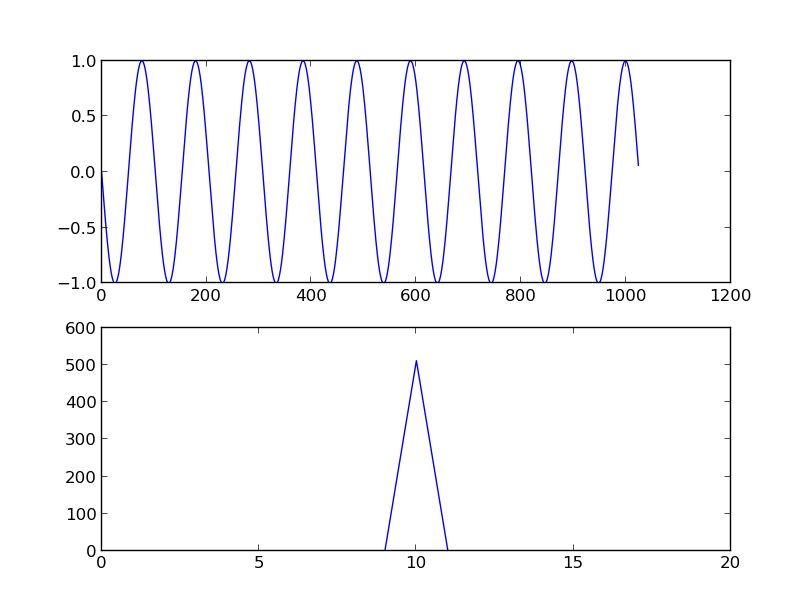
\includegraphics[width=0.9\linewidth,angle=0]{p1.png}
\caption{Problem 1.}
\label{figure1}
\end{center}
\end{figure}


\section{Problem 2}

\subsection{Description}

We analyzed the sunspot number and total solar irradiance data sets in Lecture 8. Repeat this exercise with the C02 data from Lecture 6. "Clean up" the jitters by taking the FFT, performing a manipulation, and inverse FFT, and plot the cleaned spectrum in the "time" domain again. Plot the power spectra of the data sets. 

\subsection{Result}
By setting the paddle number to be 300 and make the maxfreq=50, I manage to have the result picture: ~\ref{figure2}.



\begin{figure}
\begin{center}
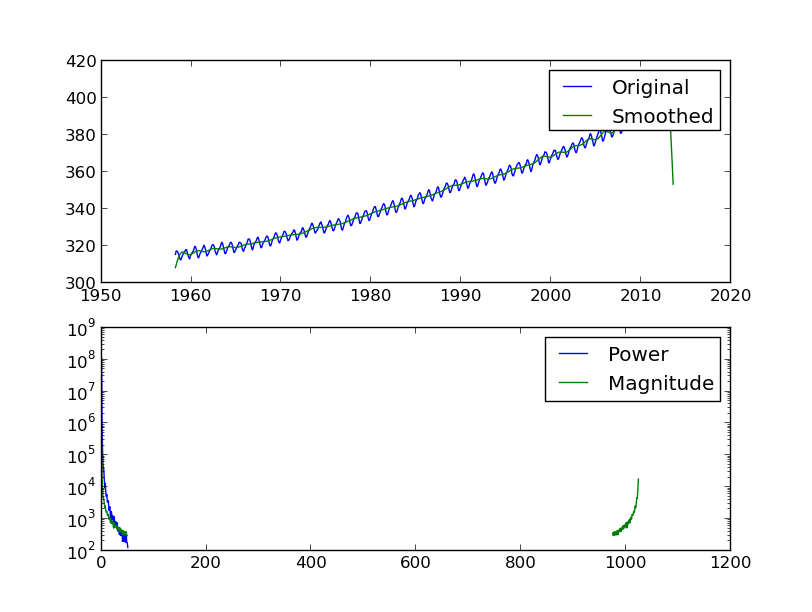
\includegraphics[width=0.9\linewidth,angle=0]{p2.png}
\caption{Problem 2 with paddle 300 and maxfreq 50}
\label{figure2}
\end{center}
\end{figure}



\section{Problem 3}
\subsection{Description}
Subtract a linear fit of the Mauna Loa CO   data from Lecture 6, and present the resulting Fourier transform. Further "clean up" the jitters by applying the "zeroing" method from class, and then plot the cleaned spectrum in the "time" domain, adding back the linear trend you subtracted earlier. 

\subsection{Result}

By doing the required steps with paddle value 0 and max frequency 50, I managed to get the result plot: ~\ref{figure3}.   



\begin{figure}
\begin{center}
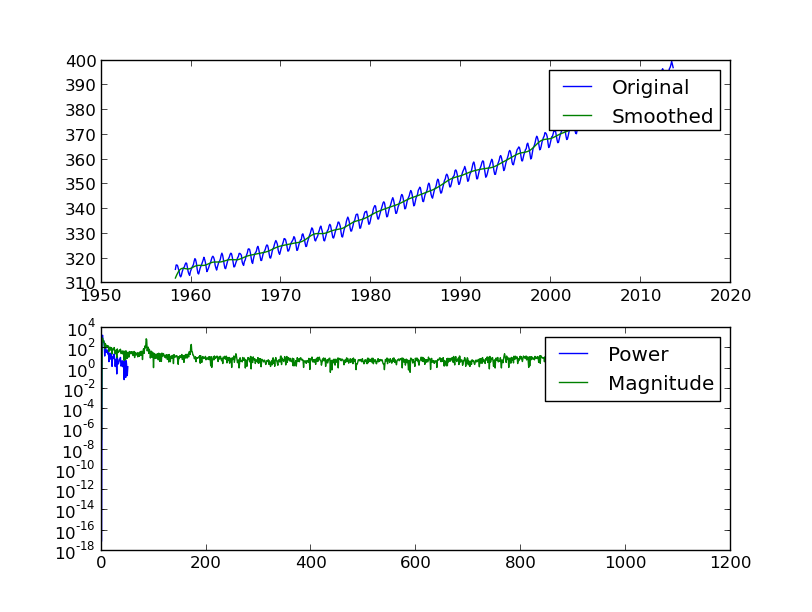
\includegraphics[width=0.9\linewidth,angle=0]{p3.png}
\caption{Problem 3 combined with linear fits }
\label{figure3}
\end{center}
\end{figure}






\newpage
\section*{Acknowledgements}

I discussed this assignment with my classmates and used material from the
cited references, but this writeup is my own.



\newpage
\appendix
\section{Appendix}

\subsection{python code}

The following python code was used to obtain the results in this report:

\lstinputlisting[language=python]{fft_test.py}

\lstinputlisting[language=python]{fft_co2.py}

\lstinputlisting[language=python]{p3_co2.py}

\end{document}
